%!TEX root=gm_jmlr.tex

We first experiment with our feature extraction algorithm \name{}-BL in the budgeted learning setting and then apply its extension \name{}-FS on feature selection problems. 

\subsection{Budgeted learning}
We evaluate \name{}-BL on two budgeted learning benchmark tasks from very different domains: the Yahoo Learning to Rank Challenge data set~\citep{chapelle2011yahoo} and the scene recognition data set from~\citet{lazebnik2006beyond}. 

\subsubsection{Yahoo Learning to Rank} 
The Yahoo Learning to Rank (Yahoo LTR) data set contains query/document pairs. Each document is a webpage document with label values from $\{0,1,2,3,4\}$. $0$ means the document is irrelevant to the query, and $4$ means it is highly relevant. In total, it has 473134, 71083, and 165660; training, validation, and testing pairs. To better simulate a real-world setting, where the irrelevant documents dominate, we follow the convention of ~\citet{chen2011} and replicate each irrelevant document (\emph{e.g.} label value is $0$) $10$ times.

Feature extraction costs are discrete values in the set $\{1, 5, 10, 20, 50, 100, 150\}$. The unit of the cost is approximately the number of limited depth regression trees that can be evaluated in the time it takes to extract the feature. The cheapest features are acquired by look-up tables, and the most expensive ones (such as BM25F-SD described in~\citet{BroGabJos10}) require time consuming term proximity scoring.

Since this data set is a ranking data set, retrieving relevant documents from a large set of irrelevant ones is most important to users. We follow the typical convention and use Normalized Discounted Cumulative Gain (NDCG@5)~\citep{jarvelin2002cumulated} to evaluate the performance. 

\textbf{Loss/cost trade-off.}
To evaluate the performance of our algorithm, we generate traces by providing different budgets. Figure \ref{fig:precision_largeset} shows the traces (dashed lines) of the NDCG@5/cost performance generated by repeatedly adding trees to the predictor until there $3000$ trees in total, simulating the results of increasing the tree-evaluation budget $B_t$. The different traces are obtained under varying values of the feature-cost trade-off parameter $\lambda$. The baseline, \emph{Gradient Boosted Regression Trees (GBRT)}~\citep{friedman2001greedy}, is cost-insensitive, and is equivalent to \name{}-BL with $\lambda\!=\!0$. Since adding too many trees results in over-fitting, we use the validation set to select the best number of trees, and this is shown in Figure~\ref{fig:precision_largeset} as red circles. We connect these red circles (the solid red line), and this trace is the performance of \name{}-BL under different budgets. As shown by the graph, the NDCG@5 ranking score drops gradually while the test-time cost budget is reduced dramatically (compared to $\lambda\!=\!0$).

\begin{figure*}[t]
\centerline{
% \includegraphics[width = .5\textwidth]{plots/prec-self}
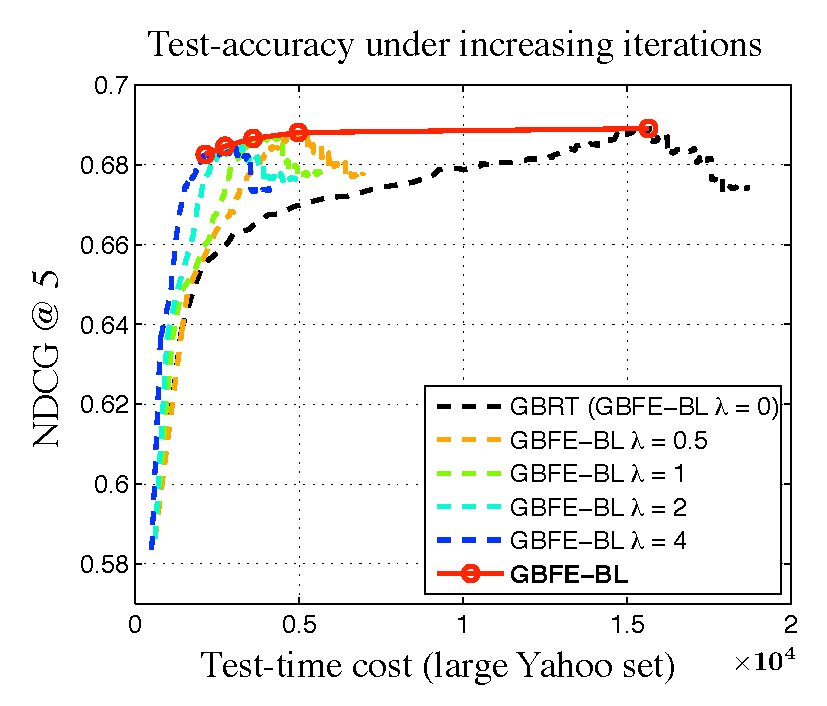
\includegraphics[width = .67\textwidth]{plots/precision_largeset}
}
\vspace{-1.5ex}
\caption{The NDCG@5 and test-time cost performance. The comparison of the original \emph{Gradient Boosted Regression Trees (GBRT) (GBFE-BL with $\lambda = 0$)} and \name{}-BL under various feature-cost/accuracy trade-off settings ($\lambda$) on the full Yahoo set. The dashed lines represent the NDCG@5 as trees are added to each classifier. The red circles indicate the best scoring iteration on the validation data set. \label{fig:precision_largeset}}
\end{figure*}

\textbf{Tuning $\lambda$.}
As shown in Figure \ref{fig:precision_largeset}, different $\lambda$ result in dramatically different performances. Each $\lambda$ corresponds to a feature extraction budget $B_f$, and if the budget is not known during training, selecting $\lambda$ could be problematic. Using a small $\lambda$ guarantees higher scores but may run over budget, using a too large one may cause under-fitting. Since \name{}-BL has a unique property that enables changing $\lambda$ at any iteration, we experiment \name{}-BL with diminishing $\lambda$ to solve the problem of unknown budget during training. Specifically, we set $\lambda$ as a function of the number of iterations $t$, $\lambda = \frac{v}{t}$, where $v$ is a certain initial value. As we gradually add more trees (increasing the number of iterations), the $\lambda$ value decreases. As shown in Figure \ref{fig:lambda}, we evaluate two different initial values ($v \in \{10, 100\}$). Compared to the baselines (fixed $\lambda = 0$ and $\lambda = 1$), the changing ones $\lambda = \frac{v}{t}$ provide smoother curves and can cope with unknown budgets during training. 

\begin{figure*}[t]
\centerline{
% \includegraphics[width = .5\textwidth]{plots/prec-self}
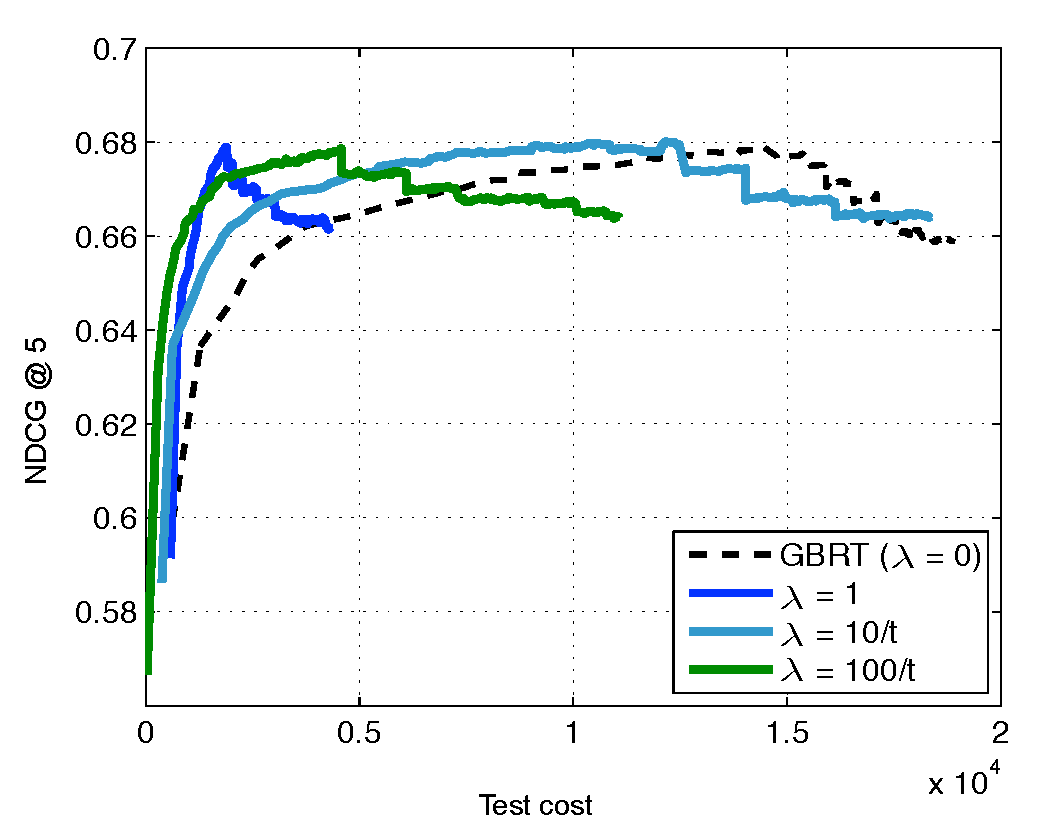
\includegraphics[width = .67\textwidth]{plots/precision_tune}
}
\vspace{-1.5ex}
\caption{The NDCG@5 and the test-time cost of various $\lambda$-settings.
The comparison of the original \emph{Stage-wise regression ($\lambda = 0$)} and \name{}-BL with fixed $\lambda$ and changing $\lambda$ on the full Yahoo set. The dashed lines represent the NDCG@5 as trees are  added to the classifier. Changing $\lambda$ at each iteration provides a smoother curve and can cope with unknown test-time budgets. 
\label{fig:lambda} }
\end{figure*}
 
\textbf{Comparison with prior work. } 
The basic baseline is GBRT, which is equivalent to \name{}-BL with $\lambda = 0$ and $3000$ trees. In addition to GBRT, we also compare against \emph{GBRT feature subsets}, \emph{Early-exit}~\citep{cambazoglu2010early} and \emph{Cronus}~\citep{chen2011}. \emph{GBRT feature subsets} is a natural cost-sensitive extension to GBRT. We first group all features according to their feature extraction cost, and train multiple regular GBRT predictors with gradually more expensive feature groups ($c_f \le 1, 20, 100, 200$). \emph{Early-exit}, proposed by \citet{cambazoglu2010early}, also builds upon GBRT. It first trains trees using regular GBRT, and then removes unpromising documents (with low prediction values) from full evaluation of the boosted ensemble (short-circuiting the sum) during test-time. Since many documents are early-exited, the average test-time cost is reduced. Among all methods of early-exit the authors suggested, we plot the best performing one (Early-exit using proximity threshold). To reduce the average test-time cost, after building all $3000$ trees, we introduce an early-exit every $10$ trees. During test-time, for the $i$th early-exit, we remove all documents that have predicted label value that is $\frac{(300-i)s}{299}$ lower than the fifth-best input. The $s$ is a parameter regulating the pruning aggressiveness, and we generate the performance curve of Early-exit by varying this parameter. The score/cost performance of Early-exit is limited because the cost is dominated by the feature extraction cost and we observe that the first $100$ trees generated by GBRT use almost all features. We also experiment \name{}-BL Early-exit described in Section \ref{sec:early-exit}. To observe the full trend of \name{}-BL Early-exit, we plot its trace as we repeatedly add trees to the predictor and we apply the exact same early-exit procedure described above (remove unpromising documents), and fix the pruning parameter $s = 0.1$.

Since Cronus~\cite{chen2011} does not scale to the full data set, we use the subset of the Yahoo data from~\citet{chen2011} of 141397, 146769, 184968, training, validation and testing points respectively, for comparison in Figure~\ref{fig:precision}. In comparison to Cronus, which requires $O(mn)$ memory, \name{}-BL requires no significant operational memory besides the data and scales easily to millions of data points.

The score and cost trade-off performances of \name{}-BL and competing algorithms are shown in Figure \ref{fig:precision}. To simulate different test-time budgets, we generate the curve of \name{}-BL by varying the feature-cost trade-off parameter $\lambda$. For each setting we choose the iteration that has the best validation NDCG@5 score. The plot demonstrates that without any budget constraints, all algorithms manage to match the highest NDCG@5 score of unconstrained GBRT. However, \name{}-BL maintains a relatively high score at much lower cost and consistently achieves higher scores than Cronus and Early-exit. In fact, \name{}-BL can almost match the ranking accuracy of stage-wise regression with 1/10 of the cost, whereas Cronus reduces the cost only to 1/4 and Early-exit to 1/2. \name{}-BL Early-exit also slightly improves over \name{}-BL.

\begin{figure*}[t]
\centerline{
% \includegraphics[width = .5\textwidth]{plots/prec-self}
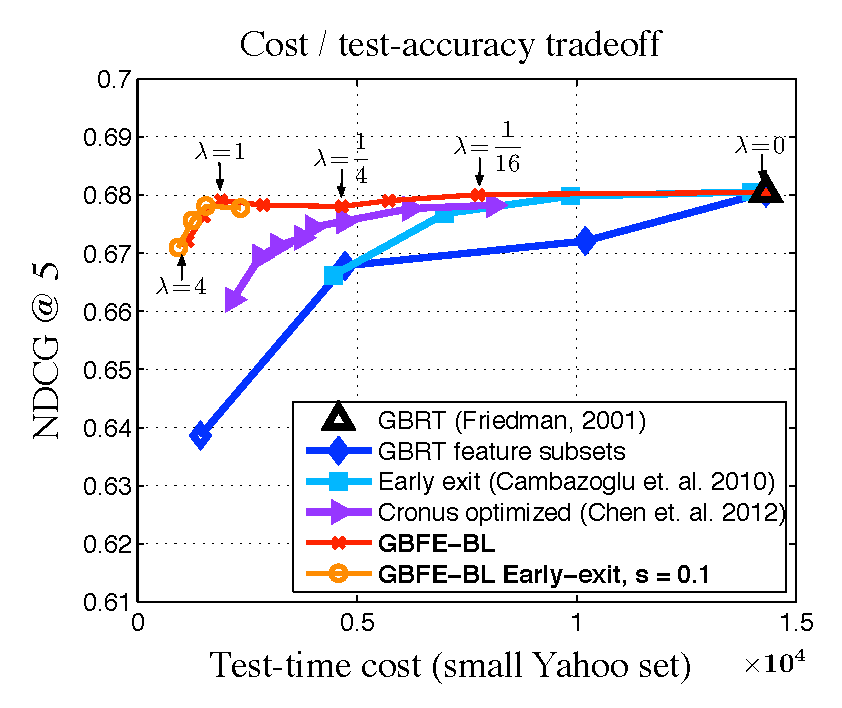
\includegraphics[width = .67\textwidth]{plots/precision_compare}
}
\vspace{-1.5ex}
\caption{Comparisons with prior work on test-time optimized cascades on the small Yahoo set. The cost-efficiency curve of \name{}-BL is consistently above prior work, reducing the cost, at similar ranking accuracy, by a factor of 10.   \label{fig:precision} }
\end{figure*}

\textbf{Feature extraction.}
To investigate the effect the feature-cost trade-off parameter $\lambda$ has on the classifier's feature extraction, Figure~\ref{fig:features} visualizes what type of features are extracted by \name{}-BL as $\lambda$ changes. For this visualization, we group features by cost and show what fraction of features in each group are extracted. The legend in the right indicates the cost of a feature group and the number of features that fall into it (in the parentheses). We plot the feature fraction at the best performing iteration based on the 
validation set. With $\lambda\!=\! 0$,  \name{}-BL does not consider the 
feature cost when building trees, and thus extracts a variety of expensive features. As $\lambda$ increases, it extracts fewer expensive features and re-uses more cheap 
features ($c_\alpha\!=\! 1$). It is interesting to point out that across all different \name{}-BL settings, a few expensive features (cost $\!\ge\!150$) are always extracted within early iterations. This highlights a great advantage of \name{}-BL over some other cascade algorithms~\citep{raykar2010designing}, which learn cascades with pre-assigned feature costs and cannot extract good but expensive features until the very end. 

\begin{figure}[t]
\centerline{
%\includegraphics[width = .5\textwidth]{plots/prec-self}
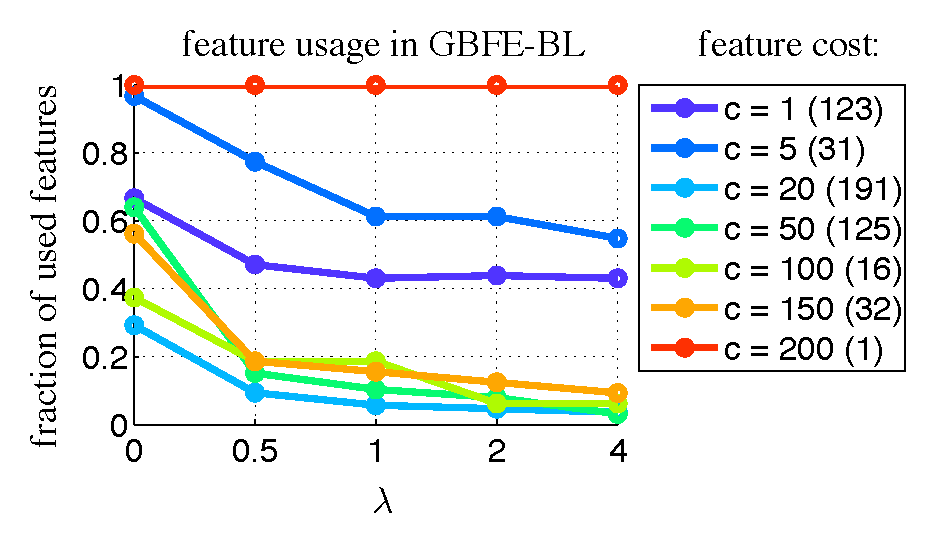
\includegraphics[width = 0.67\textwidth]{plots/features_onegraph}
}
\caption{Features (grouped by cost $c$) used in \name{}-BL with various $\lambda$ (the number of features in each cost group is indicated in parentheses in the legend). 
Most cheap features ($c\!=\!1$) are extracted constantly in different $\lambda$ settings, whereas expensive features ($c\!\geq\! 5$) are extracted more often when $\lambda$ is small. 
The most expensive (and invaluable) feature $c=200$ is always extracted.  
\label{fig:features} }
\end{figure}

\begin{figure}[t]
\centerline{
%\includegraphics[width = .5\textwidth]{plots/prec-self}
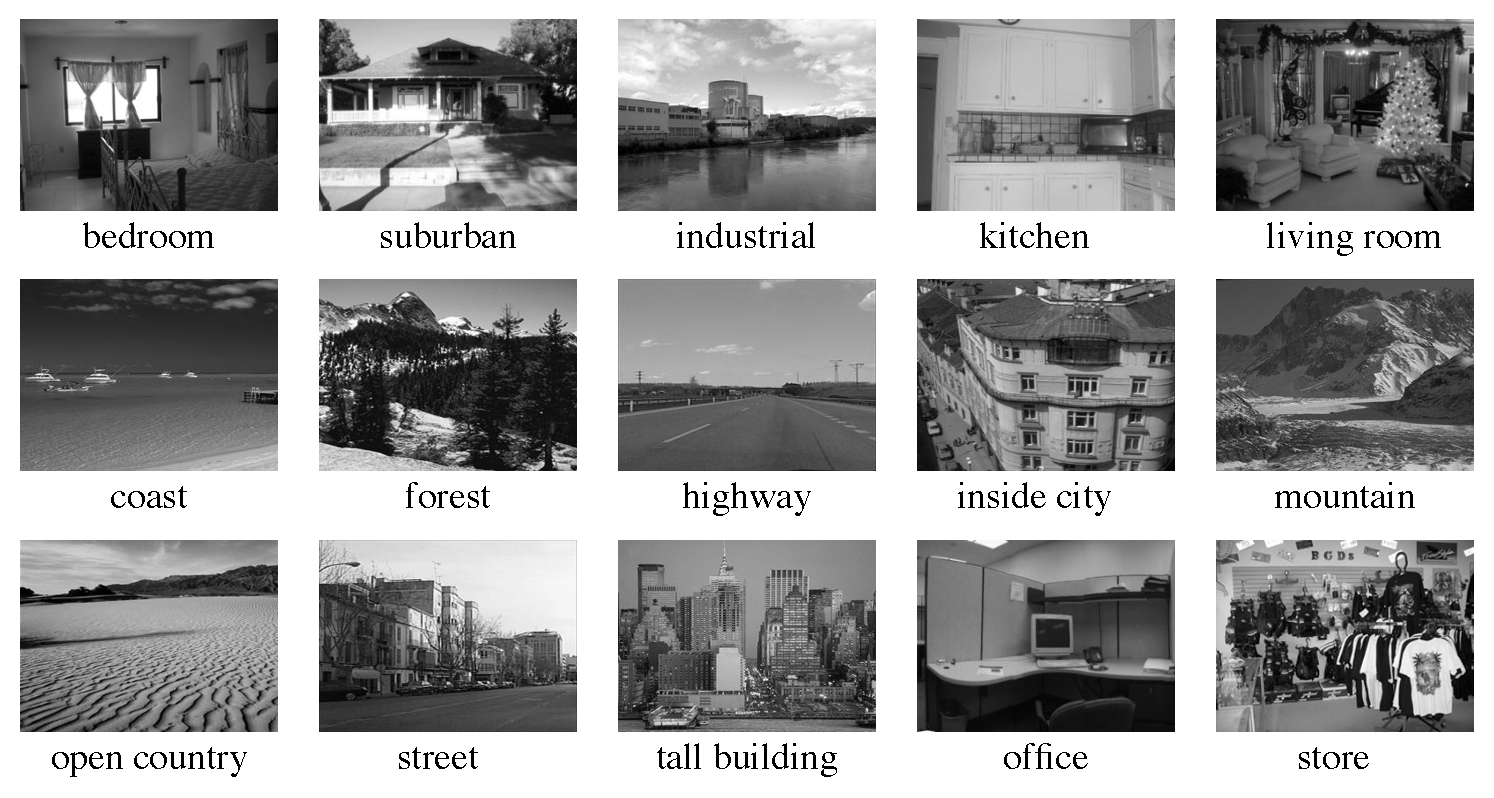
\includegraphics[width = .67\textwidth]{plots/scene15_samples_small}
}
\caption{Sample images of the Scene 15 classification task.\label{fig:sample_images}}
\end{figure}

\begin{figure}[t]
	\vspace{-1.5ex}
\centerline{
%\includegraphics[width = .5\textwidth]{plots/prec-self}
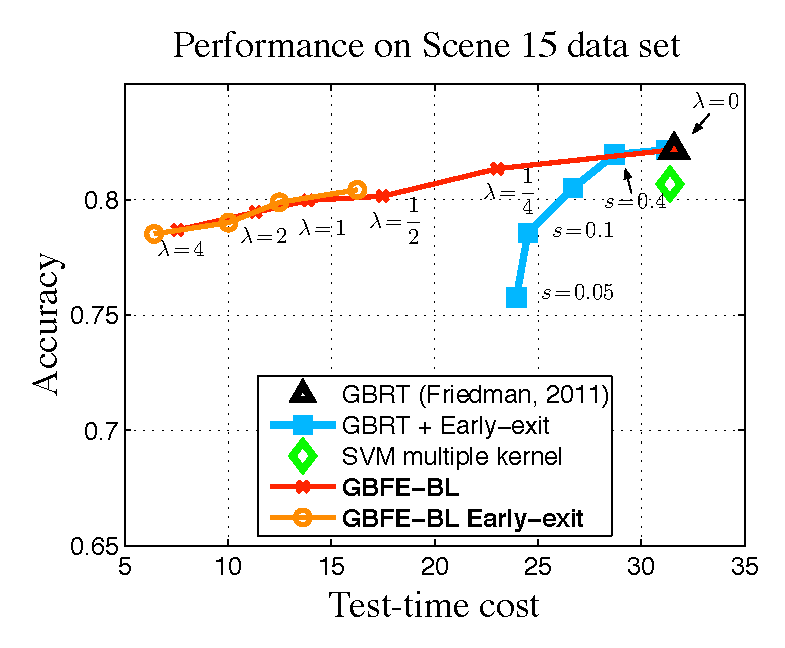
\includegraphics[width = 0.67\textwidth]{plots/scene15_noearly_depth4}
}
\vspace{-1.5ex}
\caption{Accuracy as a function of CPU-cost during test-time. The curve is generated by gradually decreasing $\lambda$. \name{}-BL offers a superior accuracy/cost trade-off and obtains similar accuracy as the SVM with multiple kernels with only half its test-time cost.  \label{fig:scene15}}
\end{figure}

% HERERE
\subsubsection{Scene Recognition} 
The second data set we experiment with is from a very different domain: scene recognition. The Scene-15 data set \citep{lazebnik2006beyond} contains $4485$ images from $15$ different scenes and the task is to classify which scene each image belongs to. Figure~\ref{fig:sample_images} shows example images from each scene category. Following the convention by \citet{lazebnik2006beyond,li2010object}, we subsample 100 images from each class for the training set. From the remaining $2985$ images, we randomly sample $20$ images from each class as a validation set, and use the rest for testing. In total, we have $1500, 300, 2685$ training, validation, and testing images respectively.


We use a diverse set of visual descriptors varying in computation time and accuracy: GIST, spatial HOG, Local Binary Pattern, self-similarity, texton histogram, geometric texton, geometric color, and Object Bank~\citep{li2010object}. Following the convention of \citet{li2010object}, we treat the $177$ object detectors within Object Bank as independent descriptors and in total, we have $7 + 177 = 184$ different visual descriptors. We then split the training set $70/30$ and use the smaller subset to train $15$ one-vs-all kernel SVM classifiers for each descriptor. We use the predictions of the larger subset as our training set features (totaling $d\!=\!184\!\times\! 15\!=\!2760$ features). To train \name{}-BL, we use the multi-class log-loss~\citep{trevor2009elements} and maintain $15$ tree-ensemble classifiers $H^1,\dots,H^{15}$, one for each class. During each iteration, we construct $15$ regression trees (depth 3) and update all classifiers. For a given image, each classifier's (normalized exponential) output represents the probability of this data point belonging to one class. 

Since generating features from different visual descriptors requires different CPU time, the feature extraction cost is naturally defined as the CPU-time required for the computation time for the visual descriptor plus the kernel computation and SVM evaluation. Each visual descriptor is used by $15$ one-vs-all features. The moment any one of these features is used, we set the feature extraction cost of all other features that are based on the same visual descriptor equal to only the SVM evaluation time  (\emph{e.g.} if the first HOG-based feature is used, the cost of all other HOG-based features is reduced to the time required to evaluate the SVM). 

Figure \ref{fig:scene15} demonstrates the performance of various algorithms on the Scene-15 data set. The basic cost-insensitive baselines include \emph{GBRT} \citep{friedman2001greedy} and \emph{SVM} with the averaged kernel of all descriptors. We also apply GBRT with \emph{Early-exit}, where we introduce an early exit every $10$ trees, and during test-time we remove test inputs with the most confident predictions (whose maximum class-likelihood is greater than a threshold $s$). We generate the curve of Early-exit by gradually increasing the value for $s$. The last baseline is multi-class logistic regression~\citep{trevor2009elements} on the original vision features with $l_1$ regularization. We notice that its accuracy never exceeds $0.74$, and therefore we do not plot it. To observe the full range of \name{}-BL, we plot the curve of \name{}-BL by varying its loss/feature-cost trade-off parameter $\lambda$, simulating different budgets. We also include \name{}-BL Early-exit by combining \name{}-BL and Early-exit  together. We use the same procedure as Early-exit described above, but fix the $s = 0.1$. As in experiments on the Yahoo LTR data set, we use the validation set to choose the best number of boosting iterations. We also average over $10$ randomly-generated train/test splits.

While both multiple-kernel SVM and GBRT achieve high accuracy, they are cost-insensitive and extract all features, resulting in a very high cost. Early-exit has very limited improvement due to the inability to select a few expensive but important features in early iterations. \name{}-BL significantly improves over all other baselines and its accuracy drops gently with increasing $\lambda$. \name{}-BL Early-exit slightly improves the cost-accuracy trade-off.

All experiments (on both data sets) were conducted on a desktop with dual 6-core 2.66GHz Intel i7 CPUs. The training time for \name{}-BL requires a comparable amount of time as GBRT (about 80 minutes for the full Yahoo data set and 12 minutes for Scene-15.)


\subsection{Feature selection}

\begin{figure}[t!!!]
\centerline{
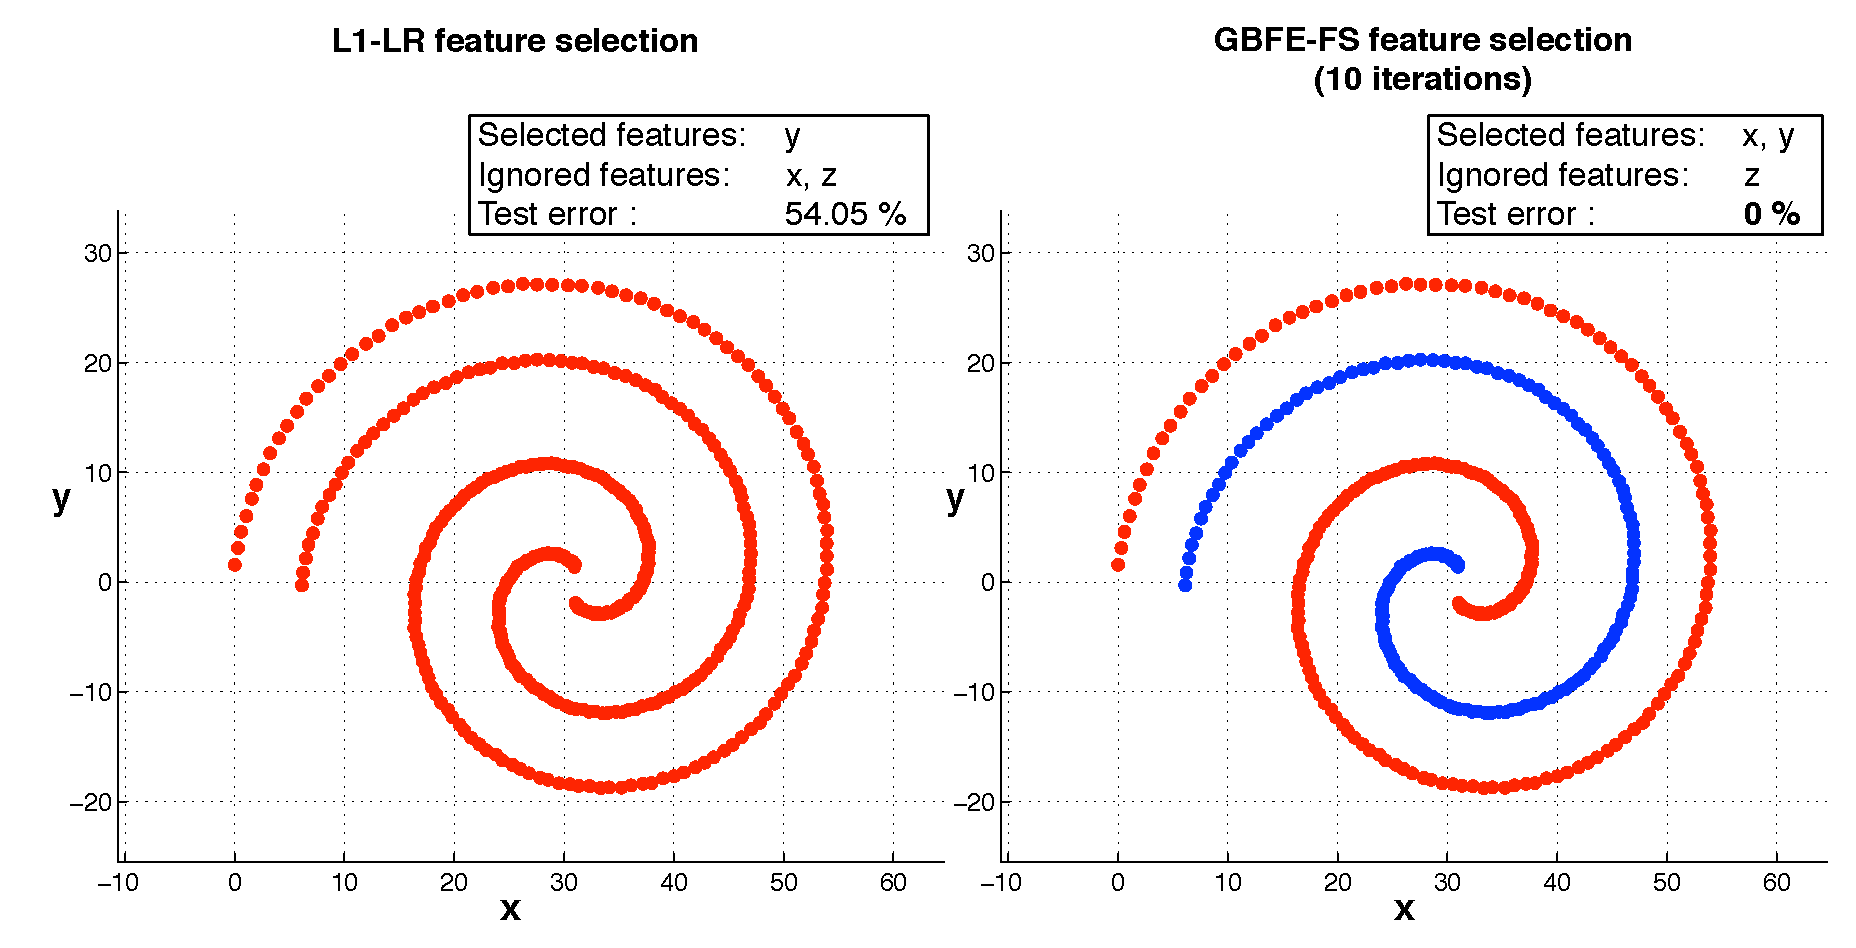
\includegraphics[width = .9\textwidth]{plots/simul}
}
\caption{Feature selection and classification performance on a simulation data set. \name{}-FS clearly outperforms the $l_1$-regularized logistic regression as it successfully captures the non-linear relations between labels and features.}
\label{fig:res_simul}
\end{figure}

In this section, we experiment with the feature selection extension of \name{}, \name{}-FS. We first evaluate it on a synthetic data set to demonstrates its unique properties, and then experiment on a bioinformatics application to evaluate its capability of selecting features with known sparsity patterns. We further compare \name{}-FS with several current state-of-the-art feature selection methods on benchmark data sets. 

\subsubsection{Synthetic data}
The synthetic data is shown in Figure \ref{fig:res_simul}. The data set is a binary classification problem and contains three features, $x$, $y$ and $z$ (where $z$ is a linear combination of $x$ and $y$, and is therefore redundant). While the data is not linearly separable in either two or three dimensions, a good \emph{non-linear} classifier should easily separate the data only based on $x$ and $y$. %The $z$ feature is a linear combination of $x$ and $y$ and is redundant. 
We randomly select $90\%$ of the instances for training and the rest for testing. 

The first baseline is \emph{$l_1$-regularized logistic regression} (L1-LR) \cite{lee2006efficient,park2007l1}. L1-LR selects features by applying an $l_1$-norm on the weight vector to produce a sparse solution. The regularization constant was set on a hold-out set. While L1-LR feature selection successfully detects the redundant feature $z$, it fails to identify a non-linear combination of $x$ and $y$ that renders good classification rates, and only selects one feature $y$. As a result, its classification error rate is very high ($54.05\%$). In contrast, \name{}-FS not only identifies the redundant feature $z$, but also detects that labels are related by a non-linear combination of $x,y$. It successfully separates the classes by selecting both $x$ and $y$ features, achieving a $0\%$ test error rate. 

\begin{figure}[t!!!]
\centerline{
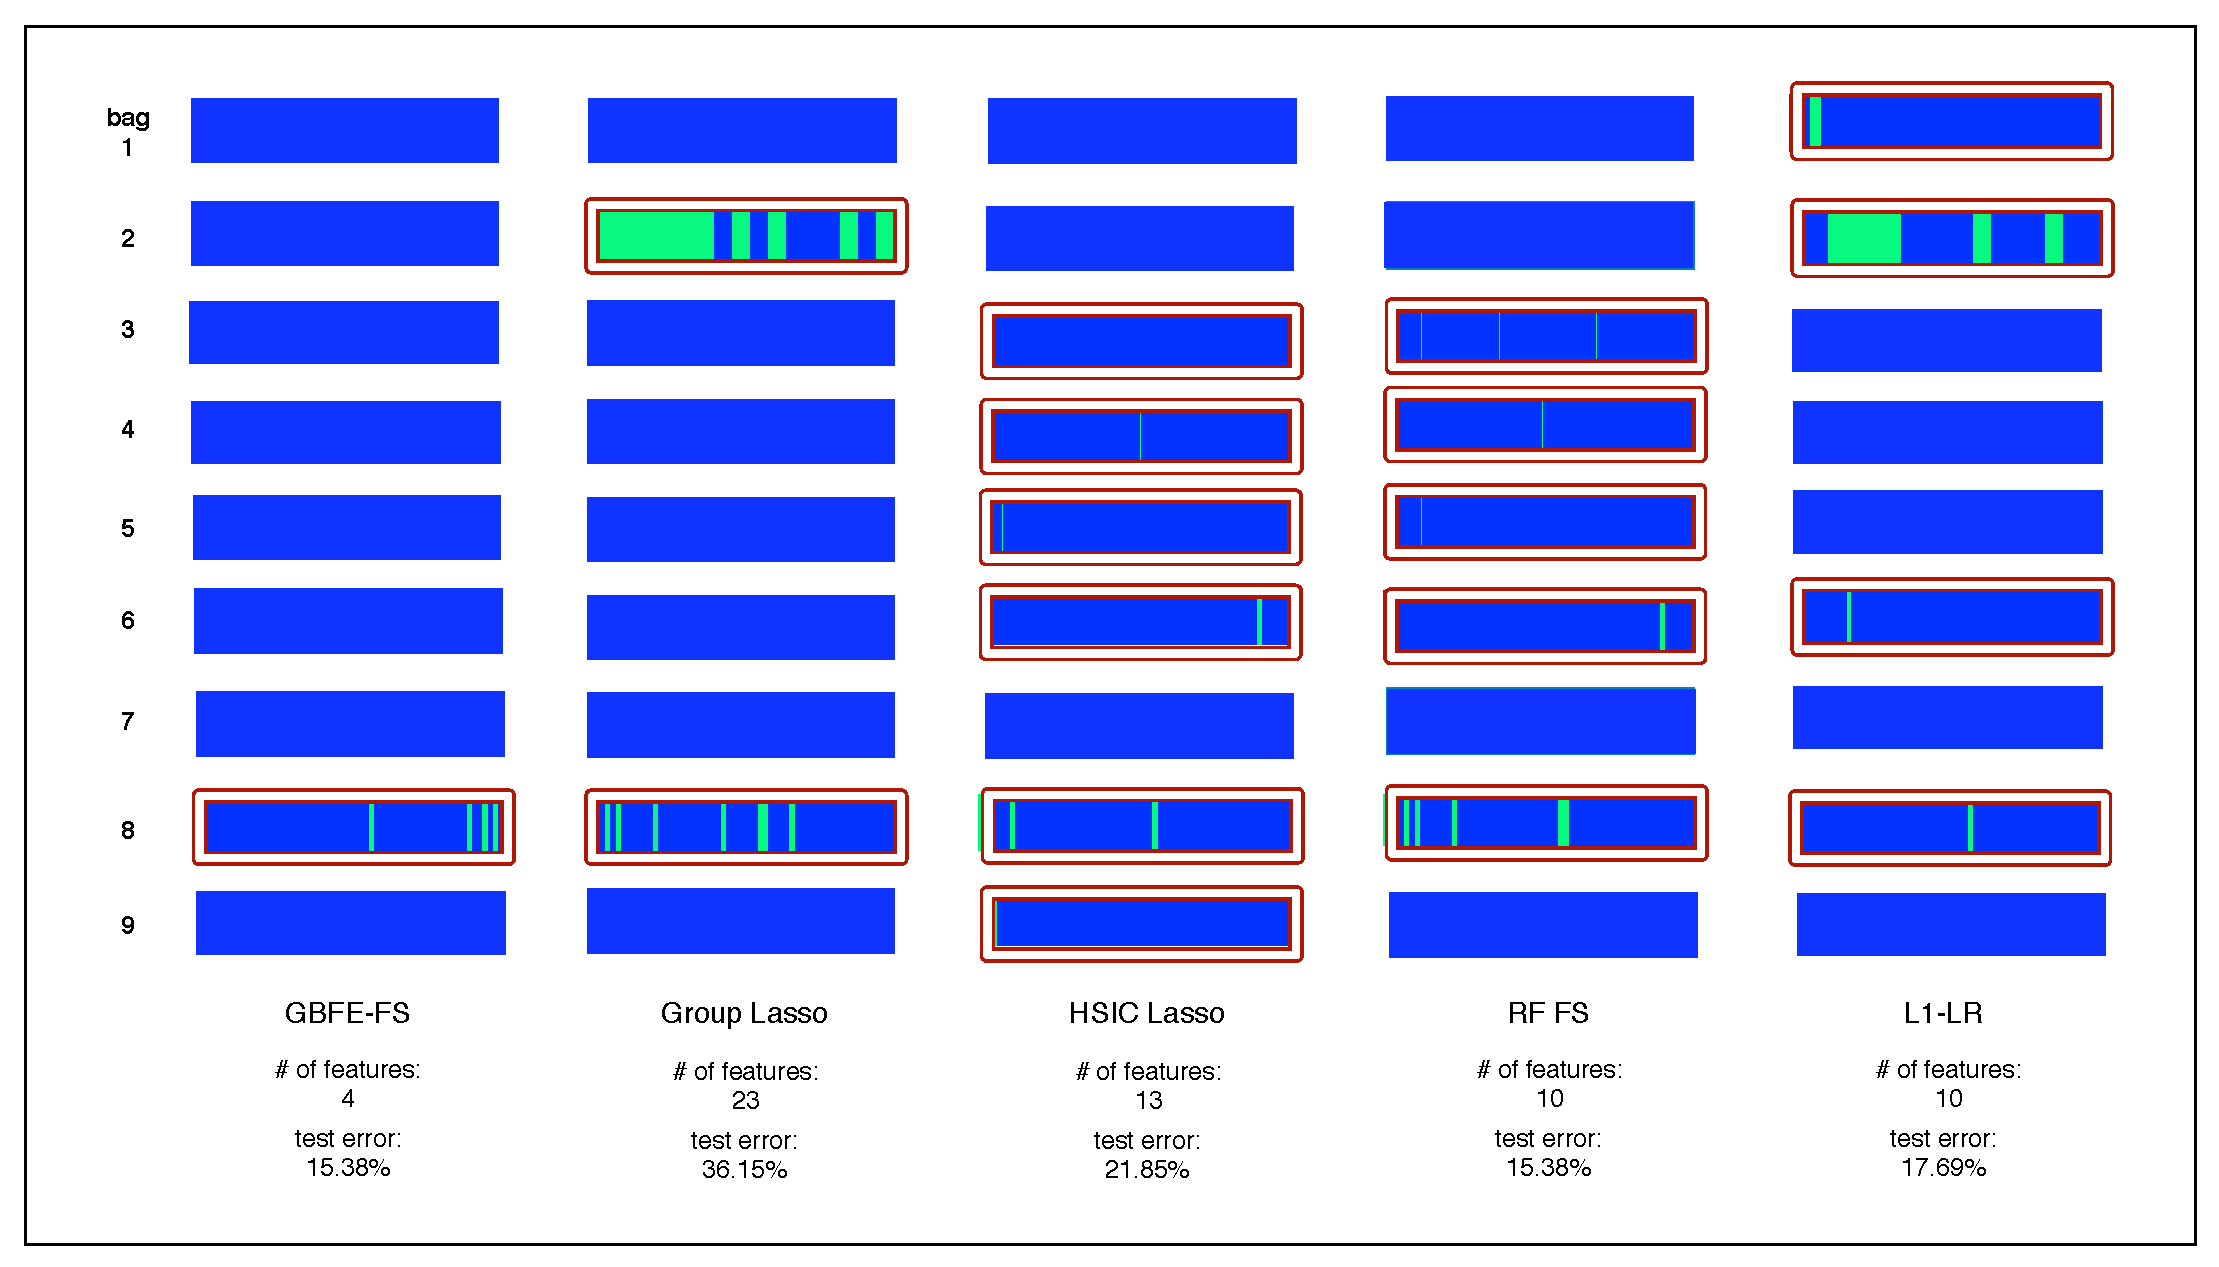
\includegraphics[width = 1\textwidth]{plots/biology_horizental}
}
% \vspace{-8pt}
\caption{Feature selection on a structured feature data set. Selected features are colored in green, and unselected are in blue. The bag is highlighted with a red/white box if at least one of its features is selected. (Some bags may require zooming in to make the selected features visible.)}
% \vspace{-10pt}
\label{fig:bag}
\end{figure}

\subsubsection{Structured feature selection}
In many real-world applications prior feature sparsity information may be provided. For example in bioinformatics or neuroscience if a classifier uses some features (such as genes or brain regions) to make predictions, it has to be biologically and neurologically explainable.

Since \name{}-FS can naturally incorporate pre-specified feature structures, we evaluate \name{}-FS for structured feature selection on the Colon data set\footnote{Available at Princeton University gene expression project: http://microarray.princeton.edu/oncology/}. In this new biology data set, $40$ tumor and $22$ normal colon tissues for $6500$ human genes are measured using Affymetrix gene chips. Among $6500$ genes, $2000$ are selected as they have the highest minimal intensity across the samples \citep{alon1999broad}. \citet{ma2007supervised} further analyze these genes and cluster them into $9$ clusters/bags according to their biological meaning. The task is to classify whether a tissue is normal or tumorous, and which cluster of genes contribute to this. We randomly split the $62$ tissues into $80/20$ training and testing datasets, repeated over $10$ random splits.
We use the feature-bag cost function $\phi_s$ mentioned in Section~\ref{sec:structure} to incorporate this side-information (setting the cost of all features in a bag to \emph{zero} once the first feature is extracted). Feature selection without considering this bag information not only performs and 
generalizes poorly, but are also difficult to interpret and justify. 

Figure \ref{fig:bag} shows the selected features from one random split and classification error rates averaged over $10$ splits. Selected features are colored in green, and unselected ones are in blue. A bag is highlighted with a red/white box if at least one of its features is selected. As for baselines, we include \emph{$l_1$-regularized logistic regression (L1-LR)}~\citep{lee2006efficient,park2007l1}, \emph{Random Forest Feature Selection (RF FS)}, \citep{trevor2009elements}, \emph{HSIC Lasso}~\citep{yamada2012high} and \emph{Group Lasso with logistic regression (Group Lasso)}~\citep{meier2008group}. 

Shown in Figure \ref{fig:bag}, \name{}-FS successfully incorporates the bag structures and focusses on selecting features from one specific bag. It selects features exclusively from bag $8$ throughout (highlighted with a red/white box in the figure). This allows the selected features to reveal the association between diseases and gene clusters/bags. Similarly, Group Lasso can also incorporate structure information. However, different from \name{}-FS, the $l_2$ regularization of Group lasso has side effects on feature weights, and thus results in a much higher error rate $36.15\%$. The rest of the algorithms: L1-LR, RF FS, and HSIC Lasso do not take bag information into consideration, and select scattered features from various bags. In terms of classification error rates, \name{}-FS matches the best performing RF FS at $15.38\%$, and out-performs L1-LR and HSIC lasso, which achieve $17.69\%$ and $21.85\%$ respectively. 

% Our explanation why \name{} can be accurate with features from only a single bag is two-fold: 1. it is indeed the case that the genes in bag $8$ are very predictive for testing if tissue is malignant or benign (a result that may be of high biological value); 2. \name{} does not penalize further feature extraction inside bag $8$ and can build a more accurate classifier than other methods, which keep penalizing all feature extractions.


\begin{table*}[t]
	\begin{center}
\begin{tabular}{|l||c|c|c|c|c|c|c|}
  \hline
  \bf{data set} & pcmac & uspst & spam & isolet & mnist3vs8 & adult & kddcup99\\
  \hline \hline
  \bf{\#training} & 1555 & 1606 & 3681 & 6238 & 11982 & 32562 & 4898431 \\ 
  \hline
  \bf{\#testing} & 388 & 401 & 920 & 1559 & 1984 & 16282 & 311029\\
  \hline 
  \bf{\#features} & 3289 & 256 & 57 & 617 & 784 & 123 & 122 \\
  \hline
\end{tabular}
	\caption{Dataset statistics. Datasets are ordered by the number of training instances.}  \label{table:datasets}
	\end{center}
\end{table*}

\subsubsection{Benchmark data sets}
In this section, we compare \name{}-FS against the current state-of-the-art in feature selection on several benchmark data sets.

\textbf{Data sets.}
Table \ref{table:datasets} lists dataset statistics ordered by increasing numbers of training instances. In this paper, we focus on a new scenario where the number of instances is much greater than the number of dimensions ($n \gg p$). While \name{}-FS can naturally extend to multi-class or regression settings, for simplicity, we convert all problems to binary classification, either by selecting the two classes that are most easily confused or (if those are not known) by grouping labels into two sets.

\textbf{Baselines.} 
The first baseline we include is \emph{$l_1$-regularized logistic regression (L1-LR)}~\citep{lee2006efficient,park2007l1}. To observe the performance of the full feature selection spectrum, we vary the regularization parameter to select different numbers of features.

We also include \emph{Random Forest Feature Selection (RF FS)}~\citep{trevor2009elements}. Similar to \name{}-FS, RF FS is a non-linear feature selection algorithm. It trains a Random Forest by building many full trees using subsets of features. It then ranks all features according to their cumulative contribution to the impurity improvement in each split, in each tree. Features with larger impurity improvement are considered more important. Throughout we run RF FS with $2000$ trees and a maximum number of $20$ instances per leaf node. After training all $2000$ trees, we rank all features. Starting from the most important features, we gradually select less important features and repeatedly re-train Random Forests with only selected features. We stop once we include all features.

The next baseline is \emph{Minimum Redundancy Maximum Relevance (mRMR)}~\citep{peng2005feature}. mRMR selects features based on their mutual information with the labels of each instance. We gradually increase the desired number of features using mRMR until we include all features. Since mRMR is not a classifier, we train an RBF kernel SVM using features selected by mRMR for classification. We tune the hyper-parameters of the SVM on $5$ different random $80/20$ splits of the training data. 

The last competing algorithm is HSIC Lasso~\citep{yamada2012high}, which is a convex extension to Greedy HSIC~\citep{song2012feature}. HSIC Lasso builds a kernel matrix for each feature, and linearly combines them to best match an ideal kernel generated from the labels. To perform feature selection, it applies an $l_1$-norm penalty on the coefficients of each kernel matrix. We evaluate a wide range of $l_1$ regularization parameters to plot the full feature selection range. Once features are selected, we train a kernel SVM with the selected features to perform classification. Similar to the mRMR experiment, we use cross-validation to select hyper-parameters and average over $5$ runs.

To evaluate \name{}-FS, we first $80/20$ split the training data into a training and validation set, and use the validation set to cross-validate two hyper-parameters (the depth of the regression trees and the number of iterations). Throughout, we fix the learning rate $\eta = 0.1$ as the model is fairly insensitive to this choice. To observe the full range of feature selection performance, we evaluate \name{}-FS with $10$ different trade-off parameters $\lambda$ (i.e., $\lambda = \{2^{-3},2^{-2},2^{-1},2^0,2^1,2^2,2^{3},2^{5},2^7,2^9\}$).

\begin{figure*}[t!!!]
\centerline{
% \includegraphics[width = 0.9\textwidth]{plots/results}
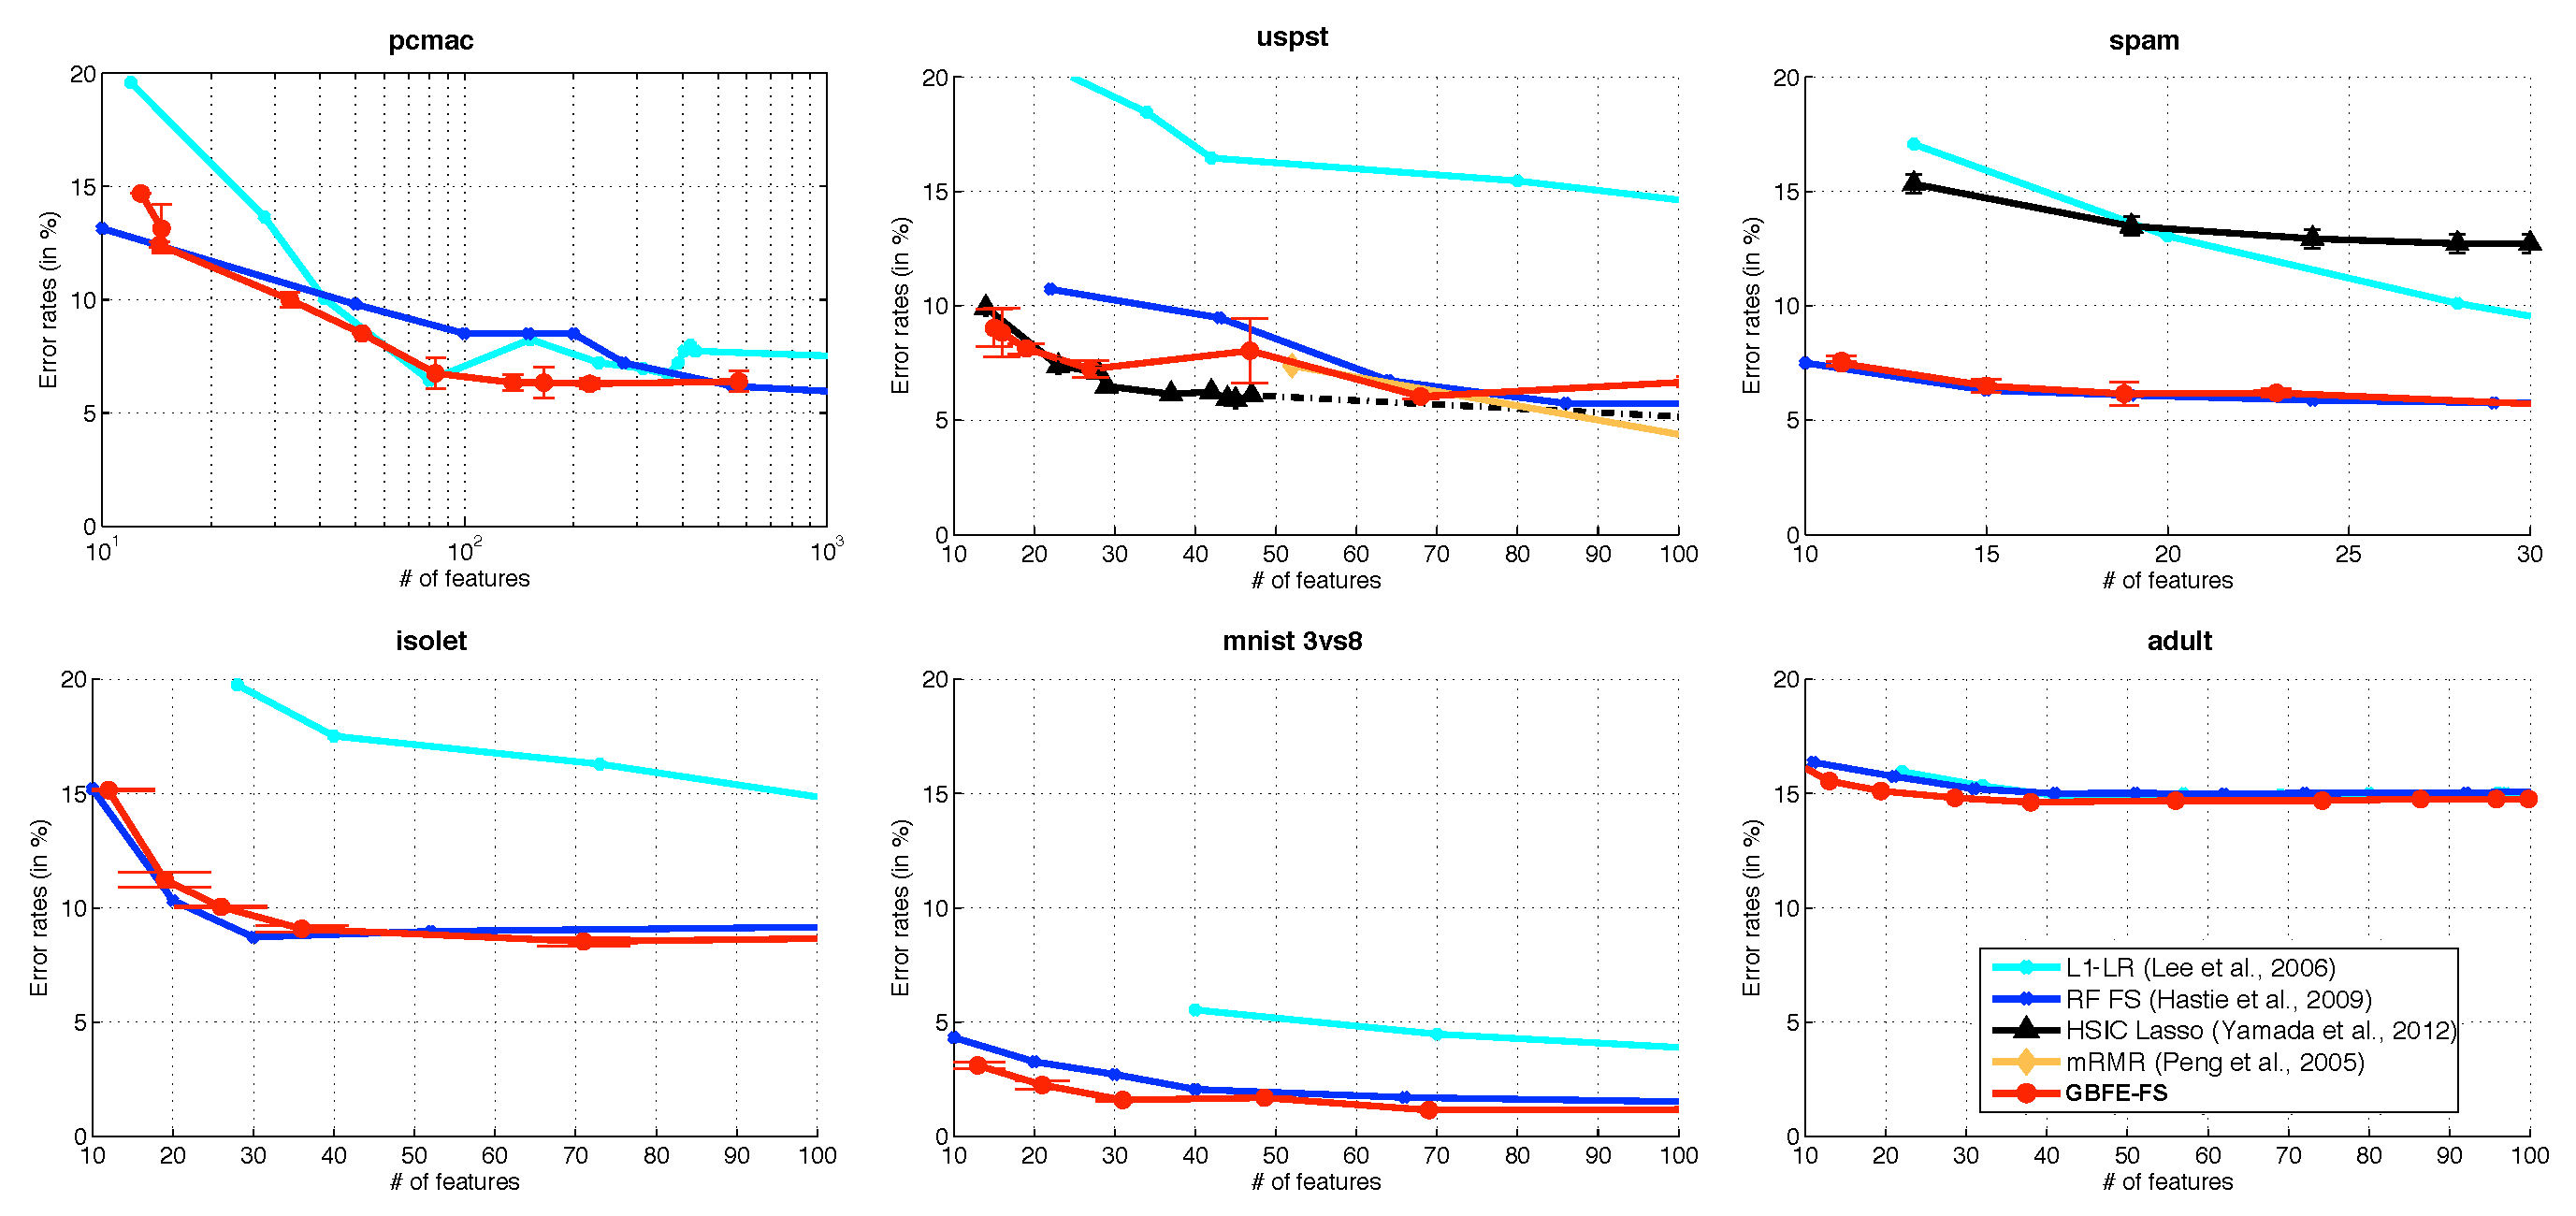
\includegraphics[width = 1.05\textwidth]{plots/results_071_100}
}
\caption{Classification error rates (in \%) vs.\ feature selection performance for different algorithms on small to medium sized datasets.}
\label{fig:results}
\end{figure*}

\textbf{Benchmark error rates.}
The performance of different algorithms on small and medium size datasets is shown in Figure \ref{fig:results}. We show the error rate levels up to 100 features except for \emph{spam} which only has $p=57$ dimensions and \emph{pcmac}, which is higher dimensional ($p=3289$). 

We observe that L1-LR, RF FS, and \name{}-FS can easily scale to all data sets. Both RF FS and \name{}-FS clearly out-perform L1-LR in accuracy on data sets because of their ability to capture non-linear feature-label correlations. HSIC Lasso and mRMR are very sensitive to the data size (both the number of training instances and the number of features), and only scale to small data sets. On small data sets where they scale, \name{}-FS still out-performs HSIC Lasso on one data set and matches mRMR. Compared to RF FS, \name{}-FS either out-performs or matches its performance on all data sets. However, one advantage of \name{}-FS is that it is a one step approach, selecting features and learning a classifier at the same time. In contrast, RF FS requires re-training a classifier after feature selection.

\begin{figure}[t!!!]
\centerline{
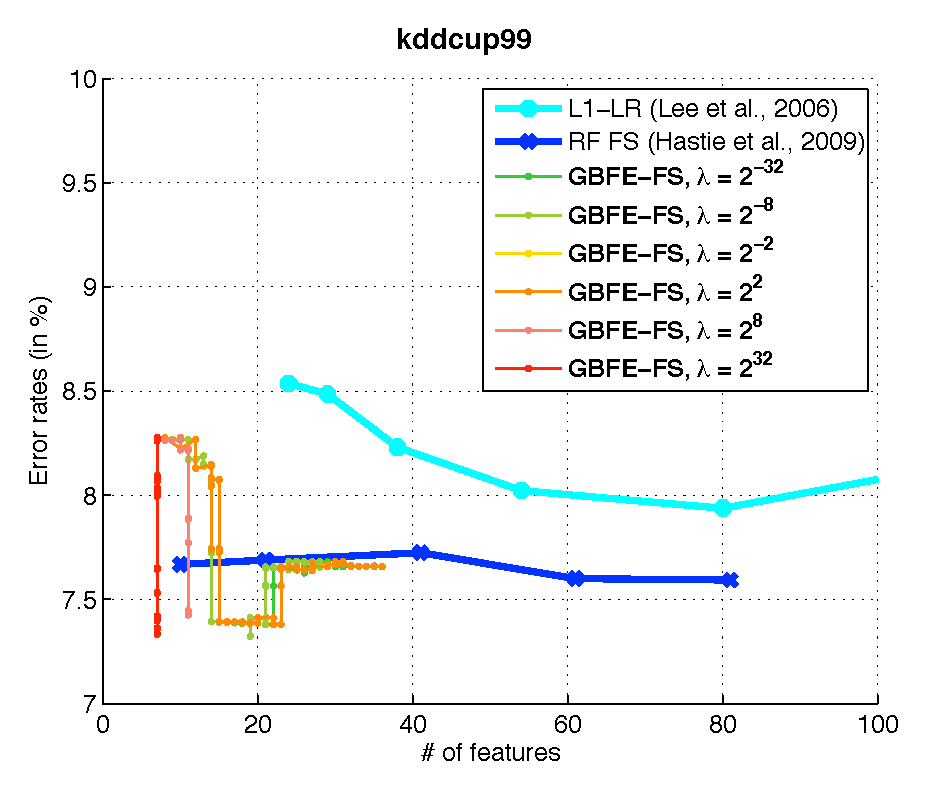
\includegraphics[width = 0.67\textwidth]{plots/largeset_071}
}
\caption{Feature selection and classification error rates (in \%) for different algorithms on the large \emph{kddcup} data set.}
% \vspace{-15pt}
\label{fig:largeset}
\end{figure}

\textbf{Massive data.}
The last data set in Table~\ref{table:datasets} (\emph{kddcup99}) contains close to 5 million training instances. Performing feature selection on such a massive dataset can be very time-consuming. We limit \name{}-FS to $500$ trees with the default hyper-parameters of tree depth $4$. Training a regular Random Forest with all default hyper-parameters would take more than a week. Therefore, we limit the number of trees to $100$ and the maximum number of instances per leaf node to $500$. As shown in Figure \ref{fig:largeset}, we plot the whole traces of \name{}-FS as we gradually add trees. Different traces are shown for different feature sparsity regularizer values $\lambda$. \name{}-FS obtains lower classification error rates than both RF FS and L1-LR when fewer features are selected. (Note that due to the extremely large data set size, even improvements $<1\%$ are considered significant).

\begin{figure}[t!!!]
\centerline{
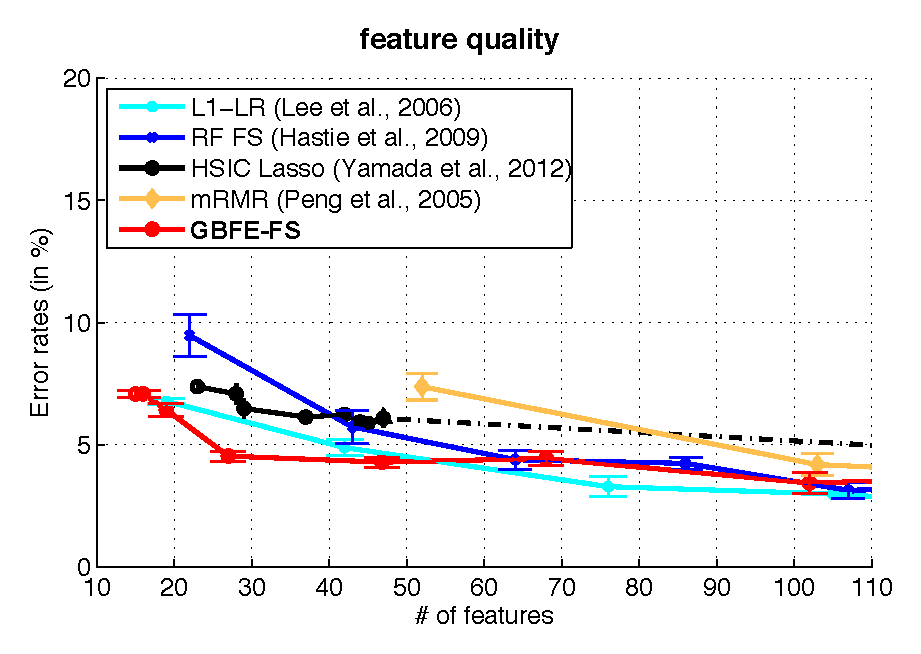
\includegraphics[width = .75\textwidth]{plots/feature_quality}
}
\caption{Error rates (in \%) of an RBF-kernel SVM trained on various feature subsets obtained with different feature selection algorithms.}
% \vspace{-18pt}
\label{fig:quality}
\end{figure}

\textbf{Feature quality.}
Since not all competing algorithms combine feature selection with classification, we separate these two tasks to further evaluate the feature selection quality of each algorithm. We run all algorithms on the smallest data set (\emph{uspst}) to select features, and then train an SVM with an RBF kernel. Figure \ref{fig:quality} shows the test error rate as a function of the number of selected features. When only a few features are selected, \name{}-FS obtains the lowest error rate. As more features are selected. all algorithms converge to similar test error. Note that the linear feature selection algorithm L1-LR out-performs most non-linear algorithms. This suggests that the \emph{uspst} digits dataset requires a non-linear classifier for classification but not for feature selection.

% \textbf{$d\gg n$ scenario.}
% While \name{} focusses on the scenario where the number of inputs is much larger than the number of features ($n\gg d$), we also evaluate \name{} on a traditional feature selection benchmark data set SMK-CAN-187~\cite{spira2007airway}, which is publicly available from~\cite{zhao2010advancing}. This binary classification data set contains $187$ inputs and $19,993$ features. We randomly select $80\%$ percent of inputs as training and $20\%$ as testing and we average over $5$ runs. Figure~\ref{fig:high_dims} shows the comparison results. \name{} out-performs $l_1$ regularized logistic regression (L1-LR), HSIC-Lasso and Random Forest feature selection (RF FS) algorithms.



% \begin{figure}[t!!!]
% \centerline{
% \includegraphics[width = 1.1\columnwidth]{plots/timing}
% }
% \caption{Training run-time for different algorithms on small to medium sizes datasets.}
% \label{fig:timing}
% \end{figure}

\subsubsection{Analysis of variance.}

\subsubsection{Computation time and complexity.} 
The fastest method so far is the linear algorithm, L1-LR. On the other hand, non-linear algorithms mRMR and HSIC Lasso are much more time consuming because their methods involve either expensive mutual information or kernel matrix computations, which scale $O(d^2)$ or $O(n^2)$. RF FS is in the middle. It builds full trees, requiring a time complexity of $O\Big(\sqrt{d}n\log(n)\Big)$ per tree, where the $\sqrt{d}$ comes from the fact that Random Forests always use a square root of number of features every time it builds a tree. 

In contrast, \name{}-FS only builds limited depth trees (depth = 4,5), and the computation time complexity is $O(dn)$. Empirically, we observe that RF FS and \name{}-FS are comparable in speed but \name{}-FS is significantly faster on data sets with many instances (large $n$). The training time ranges from several seconds to minutes on small data sets and to approximately one hour on the larger data set \emph{kddcup99} (this is the case for RF FS only if trained with only $500$ trees and large leaf sizes). 


% Unsurprisingly, the fastest method by far is  the only linear algorithm, $l_1$ regularized logistic regression.
% Both mRMR and HSIC Lasso take significantly more time than Random Forest and \name{} because they involve either mutual information or kernel matrix computation, which scales $O(d^2)$ or $O(n^2)$. Random Forest builds full trees, requiring a time complexity of $O(\sqrt{d}n\log(n)$ per tree. The  dependency on $\sqrt{d}$ is slightly misleading, as the number of trees required for Random Forests is also depended on the number of features and scales $O(\sqrt{d})$ itself.
% In contrast, \name{} only builds limited depth (depth = $4,5$) trees, and the computation time complexity is  $O(dn)$. The number of iterations $T$ is independent of the number of input features $d$ and only a function of how many features are desired to be selected.
% Empirically, we observe that the two algorithms are comparable in speed but \name{} is significantly faster on data sets with many instances (large $n$). The training time ranged from several seconds to minutes on the small data sets to about one hour on the large data  set \emph{kddcup99} (if Random Forest is trained with only 500 trees and large leaf sizes).
% Admittedly, the empirical comparison of training time is slightly problematic because our Random Forest implementation is based on highly optimized C++ code, whereas \name{} is implemented in Matlab\texttrademark. We expect that \name{} could be made significantly faster if implemented in faster programming languages (\emph{e.g.} C++) with the incorporation of known parallelization techniques for limited depth trees~\cite{tyree2011parallel}.
%Comparing training time between \name{} and Random Forests is difficult for two reasons: For Random Forest we used a highly optimized C++ optimization, whereas \name{} was implemented in Matlab\texttrademark. Further, both algorithms can be run for any number of trees, thus trading off time complexity for feature quality. Overall, Random Forests and \name{} require about the same amount of time

%Therefore, on small data sets (\emph{uspst, spam}), \name{} is $3$X faster than Random Forest, and on medium size data sets, \name{} is faster by a factor of $5$ to $10$. For the large data set \emph{kddcup99}, \name{} takes $2.2$ hours to train $500$ trees, and Random Forest takes $6.2$ hours to train $100$ trees with minimum $500$ instances in leaf nodes, which performs worse than \name{}.












